% =====================================================================
% A.L.F.R.E.D. — Bachelor Thesis
% David Zoidze · International Black Sea University (IBSU), Tbilisi
% Supervisor: Giorgi Merabishvili
% Monograph, pdfLaTeX. IBSU format: Times New Roman 12pt, 1.5 spacing,
% margins L 3cm / R 1.5cm / T,B 2.5cm, APA citations.
% Build:  pdflatex main && bibtex main && pdflatex main && pdflatex main
% =====================================================================
\documentclass[12pt,a4paper,oneside]{report}

\usepackage[utf8]{inputenc}
\usepackage[T1]{fontenc}
\usepackage{amsmath}
\usepackage{mathptmx}                   % Times New Roman (text + math)
\usepackage[left=3cm,right=1.5cm,top=2.5cm,bottom=2.5cm]{geometry}
\usepackage{setspace}
\onehalfspacing
\usepackage{graphicx}
\graphicspath{{figures/}}
\usepackage{booktabs}
\usepackage{array}
\usepackage{listings}
\usepackage{xcolor}
\usepackage{enumitem}
\usepackage[natbibapa]{apacite}         % APA author-year citations + references
\usepackage[hidelinks]{hyperref}
\usepackage{caption}
\captionsetup{font=small,labelfont=bf}

% lightweight code style for command/JSON listings
\lstdefinestyle{cmd}{
  basicstyle=\ttfamily\small,
  breaklines=true,
  columns=fullflexible,
  frame=single,
  rulecolor=\color{gray!40},
  backgroundcolor=\color{gray!5},
  keepspaces=true,
}
\lstset{style=cmd}

\title{A.L.F.R.E.D.: Adaptive Local-First Routing and Execution
Distillation for Small Language Models}
\author{David Zoidze}
\date{2026}

\begin{document}

% ---------------------------------------------------------------- front matter
\begin{titlepage}
\centering
\vspace*{1.5cm}
{\large\bfseries INTERNATIONAL BLACK SEA UNIVERSITY\par}
\vspace{0.25cm}
{\large School of Computer Science\par}
{\large COMPUTER SCIENCE PROGRAM\par}
\vfill
{\large\bfseries A.L.F.R.E.D.: Adaptive Local-First Routing and Execution
Distillation for Small Language Models\par}
\vfill
{\large David Zoidze\par}
\vspace{0.5cm}
{\large Bachelor's Thesis in Computer Science\par}
\vspace{0.5cm}
{\large Supervisor: Giorgi Merabishvili\par}
\vfill
{\large Tbilisi, 2026\par}
\end{titlepage}

\pagenumbering{roman}

% Front-matter order follows the IBSU template:
% Contents -> Acknowledgements -> Abstract -> Introduction.
% (Lists of Tables/Figures and Abbreviations intentionally omitted.)
\tableofcontents

% Acknowledgements
\chapter*{Acknowledgements}
\addcontentsline{toc}{chapter}{Acknowledgements}
I would like to express my sincere gratitude to my supervisor, Giorgi
Merabishvili, for his guidance, patience, and thoughtful feedback throughout the
development of this thesis. I am also thankful to the academic staff of the
School of Computer Science at International Black Sea University for the
knowledge and foundation that made this work possible. Finally, I am grateful to
my family and friends for their constant encouragement and support.


% Abstract (EN) — IBSU: max 1 page, in Georgian and English.
\chapter*{Abstract}
\addcontentsline{toc}{chapter}{Abstract}
On-device assistants must act on a user's behalf (setting an alarm, toggling a
setting, placing a call) without sending the request to the cloud. This thesis
asks how much language model such \emph{action} actually requires. We present
A.L.F.R.E.D., a local-first middleware that splits every request between a tiny
on-device \emph{reflexer} (a 2B model that fills a distilled command pattern in a
single forward pass) and a heavier \emph{thinker} (an agent loop) reserved for the
long tail. Across purpose-built benchmarks scored by an end-state oracle, four
results establish the central claim. First, on binding, the 2B reflexer with a
distilled pattern matches a $17\times$ larger free-form thinker (both 100\%),
while the same 2B without the pattern reaches only 30\%; distillation, not scale,
is what produces reliable execution. Second, the abstraction's benefit shifts with
the interface: on a clean settings API it is an efficiency win ($+65$ points at two
commands instead of nine), and on a realistic Android API it becomes an accuracy
win. Third, and most importantly, even a 35B reasoning model fails the device's
undiscoverable encoding conventions. Model scale buys \emph{discovery} (which key)
but not \emph{convention} (what the value means), and only a distilled pattern
supplies the convention. Fourth, that pattern can be minted automatically by a
teacher that never sees the tasks, lifting the 2B reflexer from 25\% to 76--80\%,
and the choice of teacher propagates directly to the student (a cloud teacher's
patterns score 80\% against a local teacher's 60\%). The remaining open limit is
routing, not execution. We frame these findings as the \emph{executioner
paradigm}: distill device conventions once with a strong teacher, then apply them
cheaply and repeatedly with a small on-device reflexer.

\vspace{0.6em}
\noindent\textbf{Keywords:} on-device language models, knowledge distillation,
agent routing, tool use, intent execution, privacy.


% Abstract (KA) — Georgian summary REQUIRED by IBSU. Georgian script needs
% XeLaTeX/LuaLaTeX (unavailable in this build env); text preserved in
% chapters/abstract_ka.tex. Render on a working XeLaTeX machine, or paste the
% paragraph into the final document. Re-enable the two lines below there.
% \chapter*{აბსტრაქტი}\addcontentsline{toc}{chapter}{Abstract (Georgian)}
% % Georgian abstract — machine-assisted translation of the English abstract.
% VERIFY/POLISH with a native speaker before final submission.
\begingroup\georgianfont
მოწყობილობაზე მომუშავე ასისტენტებმა მომხმარებლის სახელით უნდა შეასრულონ
მოქმედებები --- დააყენონ მაღვიძარა, შეცვალონ პარამეტრი, დარეკონ --- ისე, რომ
მოთხოვნა ღრუბელში არ გააგზავნონ. ეს ნაშრომი იკვლევს, თუ რამდენად დიდი ენობრივი
მოდელია რეალურად საჭირო ასეთი \emph{მოქმედებისთვის}. ჩვენ წარმოგიდგენთ
A.L.F.R.E.D.-ს --- ლოკალურ, ორდონიან შუამავალ სისტემას, რომელიც თითოეულ
მოთხოვნას ანაწილებს პატარა, მოწყობილობაზე მომუშავე ``რეფლექსორსა'' (2B მოდელი,
რომელიც ერთი გავლით ავსებს დისტილირებულ ბრძანების შაბლონს) და უფრო მძიმე
``მოაზროვნეს'' (აგენტური ციკლი) შორის. ოთხი შედეგი ადასტურებს მთავარ დებულებას.
პირველი: ბრძანების აგებისას 2B რეფლექსორი შაბლონით უტოლდება 17-ჯერ უფრო დიდ
თავისუფალ მოდელს (ორივესთვის 100\%), ხოლო იგივე 2B შაბლონის გარეშე აღწევს მხოლოდ
30\%-ს --- გადამწყვეტია დისტილაცია და არა მასშტაბი. მეორე: აბსტრაქციის სარგებელი
იცვლება ინტერფეისის სირთულის მიხედვით --- სუფთა API-ზე ეს ეფექტურობის მოგებაა,
ხოლო რეალისტურ API-ზე --- სიზუსტის. მესამე და მთავარი: 35B მოდელიც კი ვერ ხვდება
მოწყობილობის ``ამოუცნობ'' კონვენციებს; მასშტაბი იძლევა აღმოჩენას (რომელი გასაღები),
მაგრამ არა კონვენციას (რას ნიშნავს მნიშვნელობა), რომელსაც მხოლოდ დისტილირებული
შაბლონი ატარებს. მეოთხე: ასეთი შაბლონი შეიძლება ავტომატურად შექმნას ``მასწავლებელმა''
მოდელმა, რომელიც დავალებებს არ ხედავს, რაც 2B რეფლექსორს 25\%-დან 76--80\%-მდე
ზრდის; ამასთან, მასწავლებლის ხარისხი პირდაპირ აისახება მოსწავლეზე (ღრუბლოვანი 80\%
ლოკალური 60\%-ის წინააღმდეგ). დარჩენილი ღია შემზღუდველი არის მარშრუტიზაცია და არა
შესრულება. ნაშრომი ამ შედეგებს აყალიბებს როგორც ``შემსრულებლის პარადიგმას'': ძლიერი
მასწავლებლით ერთხელ დავადისტილიროთ მოწყობილობის კონვენციები და შემდეგ იაფად,
სამუდამოდ გამოვიყენოთ პატარა, მოწყობილობაზე მომუშავე რეფლექსორით.

\vspace{0.6em}
\noindent\textbf{საკვანძო სიტყვები:} მოწყობილობაზე მომუშავე ენობრივი მოდელები,
ცოდნის დისტილაცია, აგენტების მარშრუტიზაცია, ხელსაწყოების გამოყენება, განზრახვის
შესრულება, კონფიდენციალურობა.
\endgroup


\cleardoublepage
\pagenumbering{arabic}

% ---------------------------------------------------------------- chapters
\chapter{Introduction}
\label{ch:intro}

\section{Context}
\label{sec:context}

A growing share of what people ask a phone to do is not a question but an
\emph{action}: set an alarm, dim the screen, start a timer, turn on Do Not
Disturb, call a contact. These requests are short, frequent, and repetitive, and
they share a property that the conversational use of assistants does not. They
have a single correct outcome. Either the alarm is set for 7:00 or it is not.

How these actions are served is in the middle of an industry shift. The dominant
pattern routes a request to a large cloud model; the emerging one keeps as much
as possible \emph{on the device}. Both Google (Gemini Nano through Android
AICore) and Apple (Apple Intelligence, with Private Cloud Compute for overflow)
now run a small model locally and escalate only when they must. The motivation is
threefold: \emph{privacy}, because an action request often contains personal
context that should never leave the device; \emph{cost and latency}, because a
local model answers in milliseconds without a network round-trip or a per-call
bill; and \emph{availability}, because the device should still work offline. The
open engineering question this shift raises is the subject of this thesis: how
much language model does reliable on-device \emph{action} actually require?

\section{The problem}
\label{sec:problem}

The difficulty is a squeeze from both ends. A model small enough to run
comfortably on a phone is, on its own, an unreliable executor: asked to carry out
a device action by free-form reasoning, it either fails to act at all or invents
a command from its pretraining priors instead of the one the device expects
(Chapter~\ref{ch:eval} measures both failures). A model large enough to reason
reliably does not fit on the device, answers an order of magnitude more slowly,
costs money per call, and, as this thesis shows, is \emph{still} wrong on the
device-specific conventions that no amount of reasoning can recover.

So neither obvious option is satisfactory. Shipping a big model defeats the point
of going on-device; shipping a small free-form model is unreliable. The
interesting design space is between them: a tiny model that does not have to be
clever, paired with something that supplies the knowledge it lacks.

\section{The gap}
\label{sec:gap}

Two gaps in the existing picture motivate the work. First, the literature treats
``the model is too small'' as a single problem, when on a realistic device API it
is really two. One is \emph{discovery}: finding which setting, namespace, or key a
request maps to, which a larger model solves by exploring the API. The other is
\emph{convention}: knowing that ``total silence'' is encoded as the integer
\texttt{2}, or that ``largest font'' is the string \texttt{1.30}. Convention is
not discoverable from the API at all, because the meaning lives in a device's
accumulated conventions rather than in any queryable surface. These two
difficulties respond to completely different remedies, and conflating them hides
the most useful result in the thesis (Figure~\ref{fig:discovery}).

Second, the standard tool for compressing a capable model into a deployable one
is knowledge distillation into a smaller network's weights. That approach yields
an opaque student that must be retrained to extend. For an on-device system that
skill authors must extend and users must trust, a different distillation target
is attractive: compressing the teacher's knowledge into an \emph{inspectable,
plug-and-play symbolic artifact}. Whether such symbolic distillation is
sufficient to make a tiny model a reliable executor has not, to our knowledge,
been measured end-to-end.

\section{Thesis statement and research questions}
\label{sec:statement}

This thesis advances and defends a single claim:

\begin{quote}
On the repeatable, deterministic \emph{head} of on-device tasks, \textbf{distillation
substitutes for scale}: a 2-billion-parameter executor handed a distilled
symbolic pattern matches a $17\times$ larger free-form agent in binding accuracy,
at one on-device forward pass, because the bottleneck is not reasoning but device
knowledge the API does not expose. The remaining open limit is \emph{routing},
not execution.
\end{quote}

The claim is decomposed into five research questions, each answered in
Chapter~\ref{ch:eval}:

\begin{description}[leftmargin=2.2em,style=nextline]
  \item[RQ1 (scale vs.\ distillation)] How much model does reliable binding
    (intent $\rightarrow$ correct command) require, and can a distilled pattern
    close the gap a small model has?
  \item[RQ2 (the spectrum)] Does the value of the reflexer change with API
    difficulty: when is it an efficiency win and when an accuracy win?
  \item[RQ3 (the limit of scale)] Are there task difficulties that model scale
    cannot solve but a distilled pattern can?
  \item[RQ4 (teacher quality)] In teacher$\rightarrow$student distillation, how
    much does the choice of teacher (cloud vs.\ local) propagate to the on-device
    student?
  \item[RQ5 (coverage and routing)] What fraction of real on-device use-cases
    does the approach address, and where is the end-to-end bottleneck?
\end{description}

\section{Contributions}
\label{sec:contributions}

\begin{enumerate}[leftmargin=2em]
  \item \textbf{A two-tier local-first architecture} (A.L.F.R.E.D.) and the
    \emph{executioner paradigm}: a small reflexer treated as a constrained
    slot-filler, not a generator, with a heavier thinker reserved for the tail
    (Chapter~\ref{ch:design}).
  \item \textbf{Symbolic distillation}: knowledge distillation into a
    plug-and-play JSON pattern rather than student weights, with the
    teacher$\rightarrow$student loop measured end-to-end (Section~\ref{sec:p5}).
  \item \textbf{The discovery-vs-convention distinction}: two kinds of task
    difficulty, separated by what model scale can and cannot fix, demonstrated on
    a realistic device API (Section~\ref{sec:p4}).
  \item \textbf{Two end-state-oracle benchmarks} (SET-1 clean, SET-2
    Android-realistic) and a standardized binding-only harness, with an integrity
    protocol that forbids fabricated numbers and benchmark leakage into distilled
    artifacts (Chapter~\ref{ch:method}).
  \item \textbf{A coverage denominator} anchored to real Pixel and Apple
    on-device use-cases, and an honest localization of the open bottleneck at
    routing rather than execution (Sections~\ref{sec:coverage}--\ref{sec:routing}).
\end{enumerate}

\section{Thesis structure}
\label{sec:structure}

Chapter~\ref{ch:design} presents A.L.F.R.E.D.\ as a system: the two tiers, the
pattern artifact, the skill model, and the distillation step that connects them.
Chapter~\ref{ch:method} specifies how the system is evaluated, covering the
binding-only methodology, the end-state oracle, the benchmarks, and the integrity
rules. Chapter~\ref{ch:eval} is the core, establishing the five results above in
turn. Chapter~\ref{ch:discussion} draws out the implications for design and
productization and states the threats to validity. Chapter~\ref{ch:conclusion}
summarizes the contributions and outlines the next steps: device grounding,
deterministic value transforms, and the routing work that the evaluation
identifies as the remaining limit.
         % drafted
\chapter{Background and Related Work}
\label{ch:background}

A.L.F.R.E.D.\ sits at the intersection of four lines of work: small on-device
language models, language-model tool use and agents, model routing and cascading,
and the distillation of agent experience into reusable skills. This chapter
reviews each in turn and ends by stating precisely what gap the thesis fills. A
conceptual thread runs underneath the whole design and is worth naming first. The
two-tier split, a fast automatic path and a slow deliberate one, is the
computational analogue of two old ideas: the reflex arc, a stimulus-driven motor
response routed without higher deliberation~\citep{sherrington1906}, and the
dual-process account of cognition, in which a fast automatic system handles the
routine and a slow effortful system handles the novel~\citep{kahneman2011}. The
reflexer is the fast path; the thinker is the slow one.

\section{Small on-device language models}
\label{sec:bg-slm}

The premise that a small model is sufficient for most agentic work is now argued
directly. \citet{belcak2025slm} contend that small language models, not frontier
models, are the right substrate for agentic systems, because agent workloads are
dominated by narrow, repetitive sub-tasks that a small specialized model can serve
at a fraction of the cost. A.L.F.R.E.D.\ is a concrete instantiation of that
thesis for the on-device action setting, and supplies the mechanism (distilled
patterns) that the position paper leaves open.

On the systems side, TinyAgent~\citep{erdogan2024tinyagent} demonstrates reliable
function calling at the edge with small models, using fine-tuning and a
constrained decoder to keep a small model on the rails of a fixed tool schema.
A.L.F.R.E.D.\ shares the goal of reliable small-model tool use on-device but takes
a different route to reliability. Rather than fine-tuning the model to a schema,
it hands the model a distilled pattern at inference time, keeping the model itself
untouched and the capability set extensible by adding patterns. Industry on-device
stacks (Gemini Nano through Android AICore, and Apple Intelligence with Private
Cloud Compute for overflow) make the same architectural bet of a local small model
with selective escalation; A.L.F.R.E.D.\ is a research-grade realization of that
pattern whose tiers can be measured in isolation.

\section{Tool use and agent reasoning}
\label{sec:bg-agents}

The thinker tier implements the now-standard reasoning-and-acting loop introduced
by ReAct~\citep{yao2022react}, in which a model interleaves reasoning steps with
tool calls and observations until a task is complete. The broader line on teaching
models to use tools includes Toolformer~\citep{schick2023toolformer}, which shows a
model can learn to call APIs from self-supervised data, and
Gorilla~\citep{patil2023gorilla}, which connects a model to massive real API
collections and confronts the problem of selecting the correct call from many
candidates. These establish that capable models can use tools; the question this
thesis asks is the inverse one, namely how little model is needed once the
\emph{which-tool} and \emph{which-shape} decisions have been settled in advance by
a distilled pattern. Where ReAct spends model capability at run time to decide how
to act, the reflexer spends it once, offline, and replays the decision.

\section{Routing and cascading}
\label{sec:bg-routing}

Deciding which model or path should serve a request is the routing problem.
RouteLLM~\citep{ong2024routellm} learns to route between a strong and a weak model
from human preference data, optimizing the cost-quality trade-off;
\citet{dekoninck2024unifiedrouting} give a unified treatment of routing and
cascading and frame multi-tier systems as structured cascades, which is exactly
how A.L.F.R.E.D.'s router-then-reflexer-or-thinker path should be understood. The
difference in emphasis matters for this thesis. The routing literature largely
treats the downstream models as black boxes and optimizes the \emph{decision};
A.L.F.R.E.D.\ instead invests in making the cheap downstream path itself reliable
through distillation, and then reports honestly that the \emph{router} remains the
binding constraint on end-to-end accuracy (Section~\ref{sec:routing}). The two
concerns are complementary: a better router and a more reliable reflexer multiply
rather than substitute.

\section{Skill memory and procedural distillation}
\label{sec:bg-skills}

The closest neighbours come from work that turns agent experience into reusable
skills. Voyager~\citep{wang2023voyager} introduced the skill-library framing, in
which an agent accumulates a growing library of executable skills and composes
them; Memp~\citep{fang2025memp} studies procedural memory directly, abstracting
successful trajectories into reusable scripts. A.L.F.R.E.D.'s patterns can be read
as the deterministic compilation of exactly such procedural abstractions: where
Memp keeps scripts the agent re-interprets, A.L.F.R.E.D.\ freezes them into a
template whose only run-time freedom is slot-filling.

The Memento line is the nearest published relative. Memento~\citep{zhou2025memento}
adapts an agent without updating model weights by retrieving from a growing case
bank, a non-parametric personalization that is the same high-level strategy
A.L.F.R.E.D.\ uses with patterns. Its successor,
Memento-Skills~\citep{zhou2026mementoskills}, adds a \emph{learned} skill-router
and reflective read-write learning over free-form markdown skills. A.L.F.R.E.D.\
contrasts on two axes: its skills are \emph{compiled, deterministic} patterns
rather than free-form documents, and (as the evaluation will argue) the production
end is best served by a constrained executor whose command shape is fixed, trading
the generality of a reflective skill for the reliability of a frozen one. The
opposite design point, updating model weights to personalize an agent, is
represented by reinforcement-learning approaches such as
OpenClaw-RL~\citep{wang2026openclawrl}; this is the path A.L.F.R.E.D.\ explicitly
does not take, because weight updates sacrifice the plug-and-play, inspectable
extensibility that a symbolic pattern provides.

A note on naming is needed to avoid confusion. Our \emph{reflexer} is unrelated to
Reflexion~\citep{shinn2023reflexion}, which uses verbal self-feedback as a form of
reinforcement to improve an agent across attempts. Reflexion adds deliberation; the
reflexer removes it. The shared root word denotes opposite design intents.

\section{Knowledge distillation, classical and symbolic}
\label{sec:bg-distillation}

The mechanism that makes the cheap tier work is distillation, and its lineage is
explicit. Classical knowledge distillation compresses a large teacher network into
the \emph{weights} of a smaller student, transferring the teacher's soft behaviour
into a deployable model~\citep{hinton2015distilling}. A.L.F.R.E.D.\ distills along
the same teacher-to-student axis but changes the target: the teacher's knowledge of
device conventions is compressed into an inspectable \emph{symbolic} artifact, a
pattern, rather than into student parameters. The trade is deliberate. Weight
distillation yields a general but opaque student that must be retrained to extend;
symbolic distillation yields a student that is plug-and-play, auditable, and
composable, at the cost of covering only distilled intents. This positions the
contribution against both the distillation literature (same teacher-student idea,
different artifact) and the programmatic-prompt line such as
DSPy~\citep{khattab2024dspy}, which compiles declarative model calls into optimized
pipelines; A.L.F.R.E.D.\ similarly compiles intents into fixed command shapes, but
targets on-device execution rather than prompt-program optimization.

\section{Evaluation of agents}
\label{sec:bg-eval}

Agent evaluation has converged on task suites that score completion of realistic
multi-step goals: AgentBench~\citep{liu2023agentbench} across diverse environments,
and AssistantBench~\citep{yoran2024assistantbench} for realistic, time-consuming
web tasks. A.L.F.R.E.D.'s benchmarks share their realism goal but differ in
instrument. Rather than scoring trajectory completion, the settings benchmarks
score the \emph{end state} of a mutable backend with a no-collateral constraint
(Chapter~\ref{ch:method}), which isolates the specific failure of emitting a
plausible command that produces the wrong device state. The skill interface itself
follows the emerging \texttt{SKILL.md} convention for equipping agents with
packaged capabilities~\citep{anthropic2025skills}, with which A.L.F.R.E.D.\ is
structurally compatible.

\section{The gap}
\label{sec:bg-gap}

Across these lines, three gaps remain that this thesis addresses. First, the
small-model and routing literatures optimize the \emph{decision} of which model to
use but rarely quantify how reliable the cheap path can be made, or by what
mechanism; A.L.F.R.E.D.\ measures exactly this and finds distillation, not scale,
to be the lever (Chapter~\ref{ch:eval}). Second, the skill-memory line keeps
skills as re-interpreted scripts or free-form documents, and the consequence of
\emph{freezing} them into deterministic templates, higher reliability at the cost
of generality, has not been measured against a strong free-form baseline on a
realistic device API. Third, and most specific, no prior work separates the two
difficulties of device action, \emph{discovery} (which key) and \emph{convention}
(what the value means), then shows that model scale fixes the first but not the
second while a distilled pattern fixes both. That separation, and the
teacher-quality result that follows from it, is the contribution the remaining
chapters defend.
            % drafted
\chapter{System Design}
\label{ch:design}

This chapter describes A.L.F.R.E.D.\ as a system: the two execution tiers, the
artifacts that connect them, and the design principles that hold the whole thing
together. The goal is to fix the vocabulary that the methodology and evaluation
chapters reuse, and to make one architectural claim concrete before any number
is reported: \emph{most on-device requests do not need a model to reason; they
need a model to fill in a blank}.

\section{Overview: two tiers, one router}
\label{sec:overview}

A.L.F.R.E.D.\ sits between a user's natural-language request and the device's
capabilities. Every request enters a \textbf{router}, which makes a single
decision: can this request be served by a known, repeatable \emph{pattern}, or
does it require open-ended problem solving? The first case is dispatched to the
\textbf{reflexer}; the second to the \textbf{thinker}.

\begin{figure}[t]
  \centering
  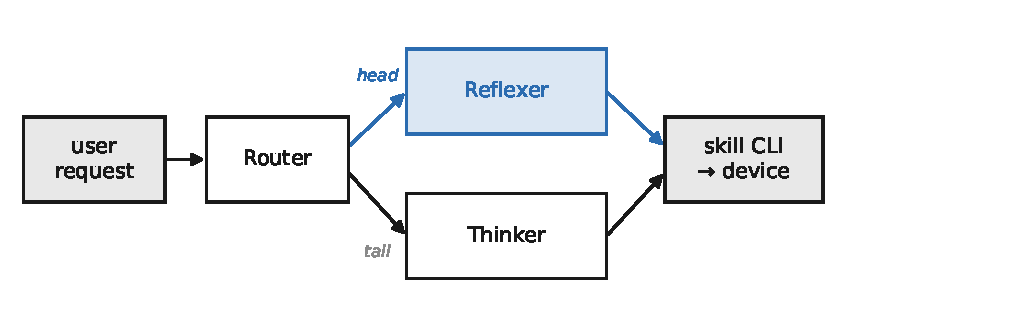
\includegraphics[width=0.95\textwidth]{fig_architecture.pdf}
  \caption{The two-tier architecture. The router classifies each request; the
  reflexer handles the deterministic head with a distilled pattern, the thinker
  handles the long tail with a full agent loop. Both emit commands to the same
  skill CLIs.}
  \label{fig:architecture}
\end{figure}

The split is an economic bet, not a capability ranking. The reflexer is cheap,
fast, and runs comfortably on the device; it is also narrow, because it can only
serve intents for which a pattern exists. The thinker is general but expensive:
it runs an agent loop, costs an order of magnitude more tokens and latency per
request, and---at the sizes that reason well---does not fit on the device at
all. Neither tier is sufficient alone. The contribution of the architecture is
the \emph{division of labour}: route the high-frequency, repeatable head to the
reflexer and reserve the thinker for the tail. Chapter~\ref{ch:eval} quantifies
exactly where that bet pays.

\section{The reflexer: an executioner, not a generator}
\label{sec:reflexer}

The reflexer is a small language model (in this work, \texttt{qwen-3.5-2b})
whose job is deliberately impoverished. It does not decide \emph{what} to do or
\emph{how} to do it. Given a request that the router has already matched to a
pattern, the reflexer extracts the variable parts of the request---the
\emph{slots}---and substitutes them into a fixed command template supplied by
that pattern. It then emits exactly one shell command. This is why we call it an
\emph{executioner} rather than a generator: it carries out a decision that was
made once, offline, by something else.

This framing is the central design choice of the thesis, and it separates
A.L.F.R.E.D.\ from the on-device assistant models shipped by Google and Apple.
Those models are asked to be creative within a constrained surface; they
generate. The reflexer is asked for none of that. It performs slot extraction
and template binding, and nothing more. The benefit is reliability: the space of
things the reflexer can get wrong shrinks to the space of slot values, because
the command shape itself is not the model's to invent. The cost is generality,
paid up front as the requirement that a pattern must exist
(Section~\ref{sec:distillation}).

Concretely, the runtime is the short pipeline in
Figure~\ref{fig:reflexer}. The matched pattern supplies a \emph{command shape}
(the \texttt{args\_template} with its slots rendered as typed placeholders) and a
list of slot descriptions; these, with the user query, form the entire prompt to
the 2B model. The model emits one shell command directly---there is no JSON step
and no separate template-rendering pass. The command is executed once through a
shell (with a per-step timeout and an optional retry), and the pattern's
\emph{validators} assert over the result. If the model errors, the command fails
to execute, or a validator rejects the outcome, the reflexer does not improvise:
it \emph{escalates} to the thinker with a tagged reason. Success is recorded; the
loop ends.

\begin{figure}[t]
  \centering
  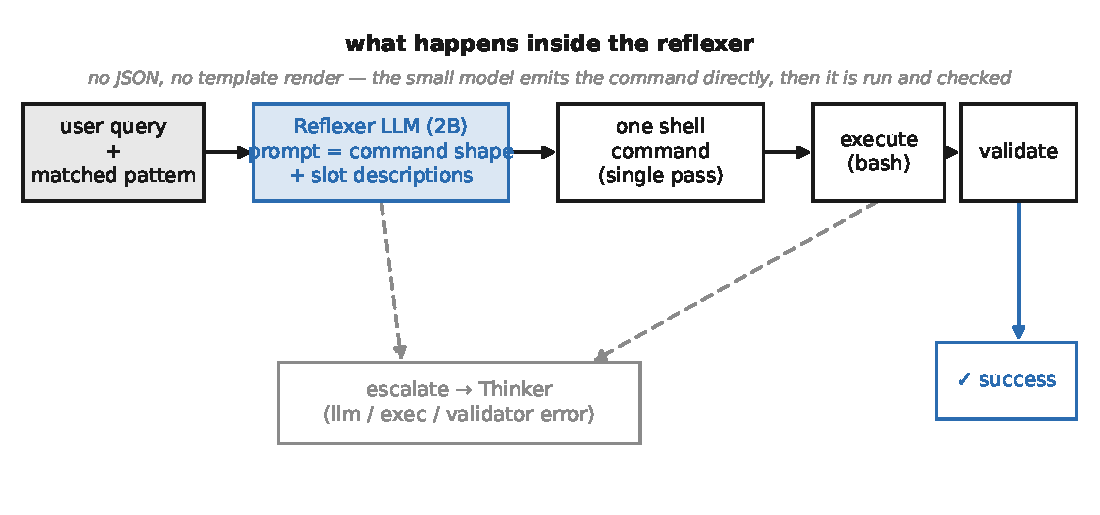
\includegraphics[width=0.98\textwidth]{fig_reflexer.pdf}
  \caption{Inside the reflexer. The pattern's command shape and slot descriptions
  prompt the 2B model, which emits a single shell command in one forward pass; the
  command is executed and validated, and any failure escalates to the thinker
  rather than being retried by reasoning.}
  \label{fig:reflexer}
\end{figure}

A single forward pass is the entire reflexer runtime. There is no tool-use loop,
no planning step. When routing is correct and a pattern exists, this
constrained executor reaches \textbf{100\% binding accuracy} on the atom task set
(Chapter~\ref{ch:eval}). The point worth stating early is structural rather than
numerical: the reflexer succeeds not because the 2B model is strong, but because
the pattern has removed almost everything it could fail at.

\section{The thinker: a general agent for the tail}
\label{sec:thinker}

The thinker is a full agent loop in the ReAct style~\citep{yao2022react}: the
model is given the relevant skill documentation and a set of tools (a shell, a
file reader), and it reasons, acts, observes, and repeats until it judges the
task complete. It is invoked for everything the reflexer cannot serve:
multi-intent or compound requests, requests requiring clarification or planning,
and any intent for which no pattern has been distilled.

Concretely, the thinker is built on the \textbf{Pi coding-agent
framework}~\citep{pi-agent}, a minimal and self-contained agent loop. Pi was
chosen deliberately: among available agent frameworks it is the simplest and most
functional---a small, transparent loop with a clean tool interface and no heavy
orchestration layer---which keeps the thinker easy to reason about and to
instrument for the binding measurements of Chapter~\ref{ch:eval}. The same
property makes Pi the intended home for future work: the planned extensions of the
reflexer (Chapter~\ref{ch:conclusion}) are to be developed inside the Pi
environment, so that the executor and the agent loop share one runtime and tool
surface.

The thinker is where capability lives, but it is also where the architecture
pays its costs. An agent loop emits many commands across several turns, consumes
substantially more tokens and wall-clock time than a single reflexer call, and
at the parameter scale required for reliable reasoning it must run off-device.
A recurring theme of the evaluation is that raw thinker capability does not
translate cleanly into reliable \emph{binding}: a free-form model, even a large
one, tends to substitute its own pretraining priors (real Linux commands,
documented backend mechanisms) for the skill's defined vocabulary. The thinker
is therefore the right tool for novel problems and the wrong tool for the
repeatable head---precisely the asymmetry the two-tier split exploits.

\section{Patterns: atoms and composites}
\label{sec:patterns}

A \textbf{pattern} is the artifact that makes the reflexer possible. It is a
small, immutable JSON record that encodes one repeatable intent. Each pattern
carries: a trigger (how the router recognizes the intent), a set of typed
\emph{slots} (the variable parts to extract from the request), an
\texttt{args\_template} (the exact command shape, with slot placeholders),
optional validators (constraints on slot values), and natural-language example
queries used by the router's embedding index.

Patterns come in two kinds. An \textbf{atom} encodes a single action---set the
screen brightness, start a timer, toggle Wi-Fi---and binds to exactly one
command. A \textbf{composite} encodes a routine made of several atoms executed in
sequence, such as a ``good night'' action that dims the screen, enables Do Not
Disturb, and sets an alarm. Atoms are the unit of reliability: they are stable,
reusable, and in our measurements essentially perfectly reflexable. Composites
are more demanding, because some require values produced at runtime (a contact
name, a URL) rather than known in advance; these remain the harder case for the
reflexer and, where they need open-ended slot extraction, are better left to the
thinker.

Critically, the \texttt{args\_template} is a \emph{hard} constraint, not a
suggestion. Where the thinker reads skill prose and may reason its way to a
different command, the reflexer is handed the command shape directly and only
fills the slots. This distinction---soft prose for the thinker versus a hard
template for the reflexer---explains much of the reliability gap between the two
tiers and is revisited in Chapter~\ref{ch:eval}.

\section{The skill model: deep modules behind a CLI}
\label{sec:skills}

A \textbf{skill} packages a device capability behind a command-line interface
and a documentation file (\texttt{SKILL.md}). The CLI is the only surface either
tier touches: the reflexer fills a template that calls it, and the thinker reads
the \texttt{SKILL.md} and invokes it through the shell. Skills emit structured
results (a JSON object reporting success, data, and errors), so that outcomes can
be checked uniformly regardless of which tier produced the command.

The skill model is an application of Ousterhout's principle of \emph{deep
modules}: a simple interface that hides substantial implementation
complexity~\citep{ousterhout2018philosophy}. A well-designed skill exposes a
small, intent-shaped vocabulary (\texttt{clock timer --duration 10m}) while
absorbing the messy device-specific mechanism behind it. This depth is what lets
even a small model act competently when it is given the right tool: on a clean,
deep settings interface the 2B reflexer succeeds on multi-step tasks that it
fails when forced to manipulate the raw state directly (Chapter~\ref{ch:eval}).
The corollary, also measured, is that a \emph{leaky} skill---one whose
documentation exposes its backend mechanism---degrades the thinker, which
reasons toward the familiar mechanism instead of the intended alias. Interface
design is therefore not cosmetic; it is a determinant of binding accuracy.

\section{Distillation: from teacher to a symbolic pattern}
\label{sec:distillation}

Patterns are not written by hand at scale; they are \emph{distilled}. A capable
\textbf{teacher} model is used once, offline, to convert a skill's documentation
and device conventions into the pattern that the cheap on-device
\textbf{student} (the reflexer) then applies forever. This is the mechanism that
pays for the reflexer's narrowness: the one-time cost of minting a pattern is
amortized over every subsequent on-device invocation.

\begin{figure}[t]
  \centering
  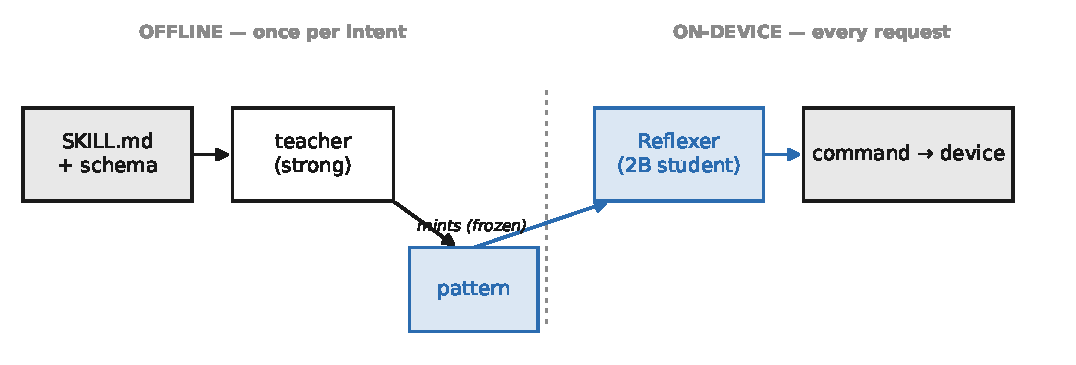
\includegraphics[width=0.95\textwidth]{fig_distillation.pdf}
  \caption{Symbolic distillation. A strong teacher reads the skill documentation
  and schema and mints a frozen JSON pattern once, offline; the cheap 2B student
  applies that pattern on-device on every subsequent request. The teacher's cost
  is paid at distillation time, not at inference time.}
  \label{fig:pipeline}
\end{figure}

The relationship to classical knowledge distillation is deliberate and worth
making precise. In the original formulation, a large teacher network is
compressed into the \emph{weights} of a smaller student
network~\citep{hinton2015distilling}. A.L.F.R.E.D.\ distills along the same
teacher$\rightarrow$student axis, but into a different target: a teacher model
compresses its knowledge of a device's conventions into an \emph{inspectable
symbolic artifact}---the pattern---rather than into student parameters. The trade
is explicit. Weight distillation yields a general student but requires
retraining to extend and is opaque to inspection. Symbolic distillation yields a
student that is plug-and-play (adding a capability is adding a JSON file, with no
retraining), auditable (the encoded convention can be read and corrected), and
composable, at the cost of covering only the intents that have been distilled.
For an on-device system that must be extended by skill authors and trusted by
users, that trade is the right one.

Two regimes of distillation appear in this work. In \textbf{cold-start}
distillation the teacher sees only the skill documentation and the API schema,
never any task or its expected outcome; it must encode each convention from
documentation and prior knowledge alone. In \textbf{session-based} (grounded)
distillation the teacher additionally observes the real device---reading back
actual setting codes before committing an encoding. Cold-start is cheaper and
captures well-documented conventions, but it cannot recover genuinely
device-specific values that no amount of reasoning can derive; those require
grounding. The boundary between what cold-start captures and what only grounding
can fix is one of the empirical results of Chapter~\ref{ch:eval}. A strict
integrity rule governs both regimes: the teacher must never see the evaluation
tasks or their gold outcomes, and a distilled pattern, once minted, is frozen
and never edited after observing failures---editing it would leak the benchmark
into the artifact under test.

\section{Design principles}
\label{sec:principles}

Three principles run through the design and are stated here because they recur as
justifications later.

\paragraph{Contract-first.} Each benchmark is specified before it is built. The
invariants (state isolation, a single success oracle, the metrics) and the
oracle itself are written down as a contract, and only then is the mechanism
implemented against that contract. This ordering prevents the common failure of
letting an evaluation drift to match whatever the system happens to produce.

\paragraph{Success is an end state, not a command.} A.L.F.R.E.D.\ is judged on
whether the device reaches the requested state without collateral changes, not on
whether it emitted a particular command string. This catches two failures that
command matching misses: a syntactically valid command that produces the wrong
outcome, and an over-eager agent that achieves the goal but also changes things
it was not asked to. The end-state oracle that enforces this is detailed in
Chapter~\ref{ch:method}.

\paragraph{Distillation is the learning phase; the reflex is frozen.} All
adaptation, iteration, and feedback live in the offline teaching step. The
runtime reflex is a single pass over a fixed pattern and never changes during
execution. This separation keeps the on-device path simple and predictable
however much effort the teacher spends producing the pattern---the analogue of a
practiced human reflex, refined slowly through feedback yet executed instantly
and without deliberation.

\bigskip
\noindent
Together these pieces define the system under test: a router that splits traffic,
a reflexer that executes distilled patterns in one shot, a thinker that handles
the tail, skills that present deep interfaces, and a distillation step that mints
the patterns offline. The chapters that follow put numbers to every claim made
here---how much model binding really needs, when the abstraction helps, where
scale stops helping, and how much the choice of teacher matters.
        % drafted
\chapter{Methodology}
\label{ch:method}

This chapter specifies how A.L.F.R.E.D.\ is evaluated, so that every number in
Chapter~\ref{ch:eval} can be read against a fixed and stated procedure. Two
methodological commitments do most of the work and are described first: scoring
only the execution stage in isolation (\emph{binding-only},
Section~\ref{sec:m-binding}) and scoring success by the resulting device state
rather than the command string (the \emph{end-state oracle},
Section~\ref{sec:m-oracle}). The benchmarks, the safeguards against runaway
agents, and the integrity rules follow.

\section{Models and infrastructure}
\label{sec:m-models}

Several models appear in the experiments, all run locally. The project began with
\texttt{ministral-3-3b} as the reflexer and later adopted \texttt{qwen-3.5-2b}
after the model sweep of Section~\ref{sec:p0}; both are used as command-generating
reflexers, and \texttt{qwen-3.5-2b} additionally serves as the small-model
\textbf{thinker} baseline. The large \textbf{thinker} is \texttt{qwen3.6-35b}, a
mixture-of-experts reasoning model (35B total, 3B active) used as the capability
ceiling for free-form binding and as a local distillation teacher. The cloud
distillation teacher is Claude Sonnet~4.6. The Qwen3.5 family at 0.8B and 4B also
appears in the reflexer sweep.

\paragraph{Serving stack and quantization.} Local models are served with
\texttt{llama-server} from \texttt{llama.cpp}~\cite{llamacpp} over its
OpenAI-compatible HTTP endpoint, and the agent loop is driven by
\texttt{pi}~\cite{pi-agent}. \textbf{All models use 4-bit (Q4) GGUF
quantization}, so that every reported number reflects a model that fits a
phone-class memory budget. The two executor models (\texttt{qwen-3.5-2b} and
\texttt{ministral-3-3b}) are served with \textbf{identical decoding parameters};
the qwen-3.5-2b invocation is reproduced verbatim in Listing~\ref{lst:serve} and
ministral-3-3b uses the same flags. The decisive settings are a low sampling
temperature ($0.2$) for near-deterministic command generation and, crucially,
\textbf{reasoning disabled} (\texttt{enable\_thinking=false})---the reflexer is an
executor, not a reasoner, so chain-of-thought is switched off. The 35B is run in
its native reasoning mode (thinking enabled), since it is evaluated precisely as
the free-form reasoning ceiling.

\begin{lstlisting}[caption={Reflexer serving configuration (\texttt{qwen-3.5-2b});
\texttt{ministral-3-3b} uses the same parameters. Q4 quantization, temperature
$0.2$, reasoning disabled.},label={lst:serve},basicstyle=\ttfamily\scriptsize]
llama-server Qwen3.5-2B-UD-Q4_K_XL.gguf --alias qwen-3.5-2b
  --host 0.0.0.0 --port 8005 --ctx-size 4072 --n-gpu-layers 999 --jinja
  --threads 16 --temp 0.2 --top-p 0.95 --top-k 20 --min-p 0.00
  --presence_penalty 0.5 --cache-type-k q8_0 --cache-type-v q8_0
  --metrics --slots --flash-attn on --cache-ram 0
  --chat-template-kwargs '{"enable_thinking":false}'
\end{lstlisting}

Runs are executed \emph{sequentially}: concurrent traffic to the same endpoint was
observed to corrupt token accounting and depress accuracy
(Section~\ref{sec:m-integrity}). Model identities, ports, and per-run parameters
are recorded with every report under \texttt{benchmark/reports/}.

\section{Binding-only evaluation}
\label{sec:m-binding}

End-to-end accuracy is the product of two stages: \emph{routing} (does the system
pick the right pattern or skill?) and \emph{binding} (given the right target,
does it emit the right command?). To measure how much model the execution stage
needs, routing must be removed as a confound. The binding-only protocol does
this by assuming perfect routing: the reflexer is handed the gold pattern for
each task, and the thinker is given the documentation for the correct skill.
Only binding is then under test. This isolation is what licenses the comparisons
in Sections~\ref{sec:p1}--\ref{sec:p2}; the cost of treating routing separately
is revisited honestly in Section~\ref{sec:routing}, where it is identified as the
real end-to-end bottleneck.

For the binding experiments, success is scored by \emph{token coverage}: a task
carries a set of gold tokens that must appear (case-insensitively) in the union
of the commands the model emitted. Both tracks read the same task files and use
the same checker---the reflexer harness
(\texttt{alfred/eval/binding\_only\_eval.py}) and the thinker harness
(\texttt{src/run-binding-compare.ts}) implement identical coverage semantics---so
that the only difference between conditions is the model and whether it received
the pattern. Standardizing the checker across both tracks was a deliberate change
to make the headline comparison fair: the reflexer is not scored by an easier
rule than the thinker.

\section{The end-state oracle}
\label{sec:m-oracle}

Token coverage is adequate for binding, where commands are short and singular,
but it is the wrong instrument for the settings benchmarks, where a request can
be satisfied by more than one command and a syntactically valid command can still
produce the wrong outcome. The settings benchmarks (SET-1 and SET-2) therefore
use a different, stricter criterion: an \textbf{end-state oracle}. Each task runs
against a mutable state backend; after the agent finishes, the oracle compares
the final state to a gold end-state and passes the task only if two conditions
hold: the requested keys reached their target values, \emph{and} no other key was
changed (no collateral edits).

This two-part definition catches two failures that command matching misses. The
first is ``right command, wrong outcome''---a command that looks correct but
leaves the device in the wrong state. The second is over-action---an agent that
achieves the goal but also changes settings it was never asked to touch, which a
command-matching scorer would happily pass. The no-collateral clause is not
hypothetical: in the distillation experiments an over-verbose pattern caused the
student to toggle extra radios, and only the end-state oracle detected it
(Section~\ref{sec:p5}). The oracle is implemented once per benchmark
(\texttt{SET-1/oracle.py}, \texttt{SET-2/oracle.py}) as the single source of
truth for success, following the contract-first principle of
Section~\ref{sec:principles}: the oracle and the task contract were written
before the runner.

\section{Sandbox isolation and the kill policy}
\label{sec:m-sandbox}

Every settings task runs in a fresh sandbox. The backend state is materialized
into a temporary file seeded with the task's initial state, the agent acts only
on that copy, and the sandbox is destroyed afterward. No task can see another
task's changes, and no run touches real device state, the network, or any
persistent user data. If an agent corrupts the state file (for example by writing
malformed JSON), the oracle reports the corruption rather than crashing, so the
failure is recorded as a failure rather than lost.

Agents that reason in a loop must be prevented from running forever. Two
mechanisms bound every run. A \emph{step ceiling} caps the number of commands an
agent may issue: for atom binding the ceiling is twice the expected number of
moves (an atom should need one command, so the cap is two), and for the
exploratory settings runs the ceiling is larger to permit genuine discovery. A
\emph{wall-clock backstop} aborts a run that exceeds a time budget regardless of
step count, which matters for the slow 35B agent. When a ceiling is hit the agent
is aborted and scored on whatever state it has produced, so a non-terminating
agent counts as a (possibly partial) failure rather than stalling the benchmark.
Both bounds, and the commands each agent actually issued, are recorded in the run
report for inspection.

\section{Benchmarks}
\label{sec:m-benchmarks}

Three benchmarks are used, chosen to bracket the difficulty of on-device action.

\paragraph{Expansion skills (binding).} Seven execution skills---clock, media,
focus, device settings, call, app, and browser---with thirty-six atoms and a set
of cross-skill composites, each backed by a mock CLI that emits a structured
result. The task set provides one to two queries per skill (the
\emph{balanced-10}) and a larger per-skill set (seventy-two atom tasks), with gold
tokens for coverage scoring. This benchmark isolates binding across a realistic
skill surface and is the basis for Sections~\ref{sec:p1}--\ref{sec:p2}.

\paragraph{SET-1 (clean settings API).} A friendly settings interface
(\texttt{settings set connectivity.wifi off}) with transparent intent-to-path
mapping and validation that rejects bad values. Twenty canonical tasks plus ten
harder multi-step tasks, scored by the end-state oracle. SET-1 isolates the value
of a deep tool on an easy surface.

\paragraph{SET-2 (realistic Android API).} An \texttt{adb}-style interface
(\texttt{settings put <ns> <key> <value>}) over thirty-two settings in three
namespaces (\texttt{system}, \texttt{secure}, \texttt{global}), with non-obvious
encodings---brightness on 0--255, timeouts in milliseconds, integer enums for Do
Not Disturb, ringer, and location, and a string-float font scale---and a
permissive \texttt{put} that silently accepts wrong inputs, exactly as the real
Android tool behaves. Forty-eight tasks, scored by the end-state oracle. SET-2 is
the realistic stressor and the setting for the limit-of-scale and distillation
results (Sections~\ref{sec:p4}--\ref{sec:p5}).

\section{Integrity protocol}
\label{sec:m-integrity}

Because the central claims rest on a handful of comparisons, the evaluation
follows explicit integrity rules, stated here so they can be checked.

\begin{enumerate}[leftmargin=2em]
  \item \textbf{No fabricated numbers.} Every figure and table cites a saved run
    under \texttt{benchmark/reports/}; no result is estimated, rounded for
    effect, or hand-edited. Where two runs of the same condition disagree, both
    are reported rather than reconciled silently.
  \item \textbf{No benchmark leakage into distilled artifacts.} In the
    distillation experiments the teacher is given only the skill documentation
    and the API schema, never any task or its gold outcome. A pattern, once
    minted, is \emph{frozen}: it is never edited after observing which tasks it
    failed, because editing it would leak the benchmark into the artifact under
    test. The frozen local-teacher patterns are committed as evidence
    (\texttt{SET-2/patterns\_distilled\_pi.json}).
  \item \textbf{Isolation.} Runs never touch real user state, never call the
    device's execution-logging path, and never use the network; each settings
    task runs in a destroyed-after-use sandbox (Section~\ref{sec:m-sandbox}).
  \item \textbf{Sequential execution.} Concurrent runs against the same model
    endpoint were found to corrupt token accounting and depress accuracy, so the
    reported runs are executed one at a time.
\end{enumerate}

These rules are the methodological backbone of the thesis: they are what allow a
small number of comparisons to carry a strong claim. The next chapter applies the
procedure defined here and reports what it found.
          % drafted
\chapter{Evaluation}
\label{ch:eval}

This chapter tests the central claim of the thesis in five steps. We first
establish how much model \emph{binding} actually needs, with routing held fixed
(Section~\ref{sec:p1}). We then explain \emph{why} a small free-form model fails
(Section~\ref{sec:p2}), and show that the value of the reflexer depends on the
difficulty of the device interface (Section~\ref{sec:p3}). Section~\ref{sec:p4}
reports the result the rest of the thesis turns on: there are task difficulties
that model scale provably cannot solve, but a distilled pattern can.
Section~\ref{sec:p5} closes the loop by distilling those patterns automatically
and measuring how much the choice of teacher matters. The last three sections
place the work in context: real-device coverage (Section~\ref{sec:coverage}),
the honest bottleneck (Section~\ref{sec:routing}), and the economics
(Section~\ref{sec:economics}).

Every number below is taken from a saved run under \texttt{benchmark/reports/};
the cited filename accompanies each result. Two evaluation disciplines hold
throughout, and are detailed in Chapter~\ref{ch:method}: \emph{binding-only}
scoring (routing assumed perfect, so that only the execution stage is under test)
and the \emph{end-state oracle} (success is the final device state, not the
command string). No number in this chapter is estimated or hand-edited.

\section{Choosing the reflexer model}
\label{sec:p0}

Before comparing tiers, the reflexer model itself must be fixed, since the rest of
the chapter holds it constant. The work began with \texttt{ministral-3-3b}, an
instruction-tuned 3B model, which already bound the deterministic slice well; the
question was whether a smaller or different model could do as well or better. We
swept the Qwen3.5 family (0.8B, 2B, 4B) against \texttt{ministral-3-3b} on the
409-atom expansion set, binding-only, each model handed the gold pattern
(\texttt{binding-only-qwen3.5-*-atoms.txt}, \texttt{binding-only-all-ministral-2026-06-16.txt}).

\begin{table}[t]
\centering
\caption{Reflexer model sweep, 409 expansion atoms, binding-only. The 2B is the
smallest model with perfect binding \emph{and} perfect vocabulary compliance.}
\label{tab:reflexer-sweep}
\begin{tabular}{lcc}
\toprule
Model (Q4) & Atom binding & Signature failure mode \\
\midrule
qwen-3.5-0.8b & 380/409 (92.9\%) & violates vocabulary (emits \texttt{docker}, not the \texttt{dock} alias; 0\% docker) \\
\textbf{ministral-3-3b} & 391/409 (95.6\%) & prunes static flags (\texttt{-{}-skip-download}; youtube 81\%) \\
\textbf{qwen-3.5-2b} & \textbf{409/409 (100\%)} & none \\
qwen-3.5-4b & 100\% on captured subset$^{\dagger}$ & none observed \\
\bottomrule
\end{tabular}

\smallskip
{\footnotesize $^{\dagger}$ A full 409-run for 4B was not persisted (only a
docker+service subset, 24/24); it is not reported as a full figure. On the larger
627-task set including core skills, ministral-3-3b scores 601/627 (95.9\%).}
\end{table}

Two findings come out of the sweep. First, \texttt{qwen-3.5-2b} is the best
reflexer found: perfect binding across all 409 atoms, beating both the smaller
0.8B and the larger ministral-3-3b, at the smallest size that fits a 4\,GB device
budget, so it is adopted for the rest of the thesis. Second, and more
interesting, the small models fail in \emph{model-specific signatures} rather than
a single universal weakness. The 0.8B is \emph{semantically} correct but
\emph{schema}-noncompliant: it emits the real binary name (\texttt{docker start})
instead of the skill's defined alias (\texttt{dock start}), failing every docker
task even at temperature $0.2$, because it cannot override a strong lexical prior.
The 2B complies perfectly, at parity with 4B. Vocabulary compliance is therefore a
\textbf{capability threshold between 0.8B and 2B} rather than a smooth gradient,
and scale beyond 2B buys nothing here. The ministral-3-3b signature is different
again: it obeys the vocabulary perfectly but prunes semantically-secondary static
flags (\texttt{-{}-skip-download}), which is why a capable 3B nonetheless drops to
81\% on the affected skill. The lesson for the design is that a reflexer must be
chosen for \emph{schema obedience}, not raw capability, and that a 2B model already
clears that bar.

\section{The binding spine: distillation substitutes for scale}
\label{sec:p1}

The first experiment fixes routing and asks a single question: given that the
right intent has been identified, how large must a model be to emit the right
command? We compare three conditions on the same matched task set (the
\emph{balanced-10}: one to two tasks per skill across all seven skills):
a 2B reflexer handed the distilled pattern, and a free-form thinker (given only
the skill documentation) at 2B and at 35B.

\begin{table}[t]
\centering
\caption{Binding accuracy on the matched balanced-10 set, with routing held
fixed. The 2B reflexer with a pattern equals the 35B free-form thinker; the same
2B without the pattern reaches only 30\%.}
\label{tab:spine}
\begin{tabular}{lcccc}
\toprule
Condition & Binding & Model size & Median latency & Tokens/task \\
\midrule
Reflexer + pattern & \textbf{10/10 (100\%)} & 2B & single call & n/a (1 call) \\
Thinker, no pattern & \textbf{10/10 (100\%)} & 35B & 6.4 s & $\sim$1.3k \\
Thinker, no pattern & 3/10 (30\%) & 2B & 1.7 s & $\sim$0.7k \\
Thinker, no pattern & 1/10 (10\%) & 4B$^{\dagger}$ & 2.8 s & $\sim$0.7k \\
\bottomrule
\end{tabular}

\smallskip
{\footnotesize $^{\dagger}$ The 4B is configured at context 4000 versus the
35B's 131k, so its thinking crowds the skill document; it is not a clean
capability point. Sources: \texttt{binding-only-phase2-qwen2b-balanced10.txt},
\texttt{thinker-binding-phase2-qwen35b-balanced10.txt},
\texttt{thinker-binding-phase2-qwen2b-balanced10.txt},
\texttt{thinker-binding-phase2-qwen4b-balanced10.txt}.}
\end{table}

\begin{figure}[t]
  \centering
  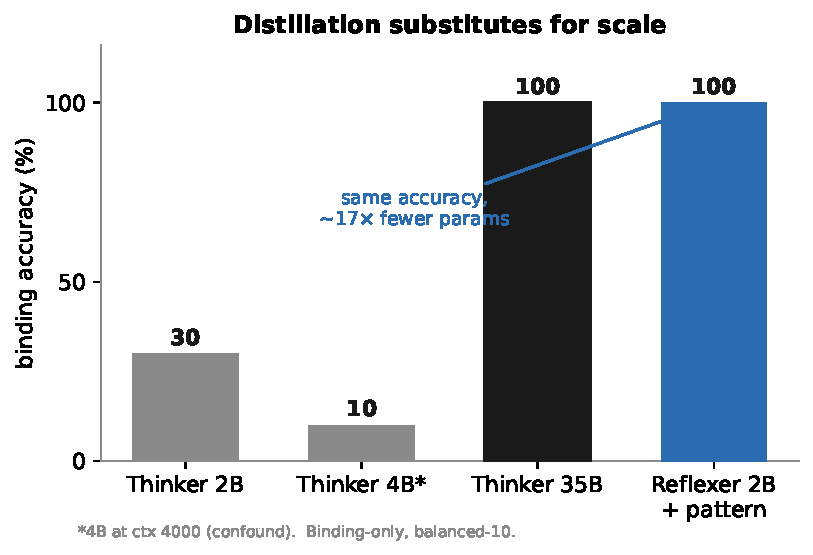
\includegraphics[width=0.72\textwidth]{fig_binding.pdf}
  \caption{Binding accuracy by condition (balanced-10). Scale alone is
  non-monotonic (4B $<$ 2B $<$ 35B); the pattern takes a 2B to the 35B ceiling.}
  \label{fig:binding}
\end{figure}

The result, stated plainly: \textbf{a 2B reflexer with a distilled pattern
matches a 35B free-form thinker (both 100\%), while the same 2B without the
pattern manages 30\%}. The pattern is worth roughly $17\times$ the parameters on
this task. The effect persists at scale on the full set: the 2B reflexer binds
\textbf{72/72 (100\%)} atoms across every skill, where the 2B thinker manages
only \textbf{14/72 (19.4\%)} (\texttt{binding-only-phase2-qwen2b.txt},
\texttt{thinker-binding-phase2-qwen2b.txt}).

Two readings must travel with this headline. First, scale is an \emph{unreliable}
lever for binding: the 4B scores below the 2B, partly a context confound but
partly a real signal, in that the 4B emits higher-quality \emph{real} Linux
commands (\texttt{nmcli radio wifi off}, \texttt{playerctl pause}) because it knows
the true APIs better, and so obeys the skill's defined surface \emph{less}.
Capability to know and obedience to the surface can trade off. Second, this is a
systems and efficiency result, not a claim that ``2B is smarter than 35B.'' The
reflexer is handed the command template and only fills slots, a strictly easier
task than free-form generation. The legitimate claim is precise: \emph{on the
deterministic slice where intents repeat often enough to distill, a 2B constrained
executor matches a 35B free-form thinker's binding accuracy at a fraction of the
size, latency, and tokens.}

\section{Why the small free-form model fails}
\label{sec:p2}

The 30\% of the unaided 2B thinker is not uniform incompetence; it decomposes
into two distinct and opposite failure modes, visible when the per-skill numbers
are examined (\texttt{thinker-binding-phase2-qwen2b.txt}): app 0/6, browser
0/16, call 0/8, clock 1/14, focus 1/6, media 3/10, and device\_settings 9/12.

\paragraph{Under-triggering (no action at all).} On all eight \texttt{call}
tasks the 2B thinker emitted \emph{zero} commands. Short social imperatives such as
``call mom,'' ``hang up,'' and ``answer'' hit the model's conversational prior, and
it replies in prose instead of invoking a tool. With no command emitted, the task
is an automatic miss. The failure is not wrong output; it is the absence of
output.

\paragraph{Wrong vocabulary (real-shell substitution).} On \texttt{app} tasks the
model \emph{does} act, but free-forms from its pretraining prior: \texttt{spotify
\&}, \texttt{killall firefox}, \texttt{ps aux | grep}, never the skill's defined
\texttt{app open -{}-name}. Capability is present; obedience to the defined
surface is absent.

The diagnostic skill is \texttt{clock}, whose documentation deliberately exposes
its real backend (\texttt{systemd-run}, \texttt{systemctl}). Here even the 35B
thinker binds only 30\% (\texttt{thinker-binding-phase2-qwen35b-first10.txt}),
and the 2B only 7\% (1/14), while the reflexer binds 100\% (14/14). A reasoning
model reads the leaked mechanism and prefers the concrete tool it has a strong
prior for (\texttt{systemctl -{}-user list-timers}) over the abstract
\texttt{clock} alias it has a weak prior for. For the thinker, the skill document
is a \emph{soft} prompt mediated by priors and sampling; for the reflexer, the
\texttt{args\_template} is a \emph{hard} constraint with no prose to reason
around. Both failure modes are erased by the pattern, which hard-codes the
command shape. This is also a productization argument for distillation: the
reflexer is robust to documentation quality, whereas the thinker is not.

\section{The spectrum: efficiency on clean APIs, accuracy on realistic ones}
\label{sec:p3}

Whether the reflexer's benefit shows up as \emph{efficiency} or as \emph{accuracy}
depends on the interface. Two settings benchmarks bracket the range. SET-1 is a
clean, friendly settings API (\texttt{settings set connectivity.wifi off}); SET-2
is a realistic Android API (\texttt{settings put <ns> <key> <value>}) with three
namespaces, non-obvious encodings (brightness 0--255, timeouts in milliseconds,
integer enums for Do-Not-Disturb and location, a string-float font scale), and a
permissive \texttt{put} that silently ``succeeds'' on wrong inputs, exactly how
\texttt{adb shell settings} behaves.

On the \emph{clean} API the small model is already a competent executor when it
is given a deep tool (Table~\ref{tab:set1}). Manual state editing collapses to
about a third; the same model driving the deep \texttt{settings} script reaches
100\%, including two- and three-step compound tasks, because the script rejects
wrong guesses and the model recovers. The gain is real, but it is
\emph{efficiency and competence} (fewer calls, fewer tokens, recovery from
error), not new accuracy the model lacked.

\begin{table}[t]
\centering
\caption{SET-1 (clean API), qwen-3.5-2b. The deep tool is an efficiency win:
$+65$ percentage points, at 2 calls instead of 9. Sources:
\texttt{set1-e1e2-qwen2b.txt}, \texttt{set1-e2-hard-qwen2b.txt}.}
\label{tab:set1}
\begin{tabular}{lccc}
\toprule
Mode & Oracle pass & Median calls & Median tokens \\
\midrule
E1, manual JSON edit (no script) & $\sim$30--35\% & 9 & 3098 \\
E2, \texttt{settings} script & \textbf{100\%} (20/20; hard 10/10) & \textbf{2} & \textbf{775} \\
\bottomrule
\end{tabular}
\end{table}

On the \emph{realistic} API the picture inverts. A free-form 2B thinker over the
48 SET-2 tasks scores \textbf{12/48 (25\%)} (\texttt{set2-thinker-qwen2b-48.txt}).
Its failures cluster exactly on what cannot be guessed: every brightness percent
that must become 0--255, every timeout that must become milliseconds, the integer
enums, and the key-name traps (\texttt{airplane mode} $\rightarrow$
\texttt{airplane\_mode\_on}). It passes only guessable booleans and trivial
arithmetic. Here the abstraction is no longer about efficiency: a small free-form
agent simply \emph{cannot} drive a realistic device-settings API. The reflexer's
benefit has shifted from saving calls to supplying accuracy.

\begin{figure}[t]
  \centering
  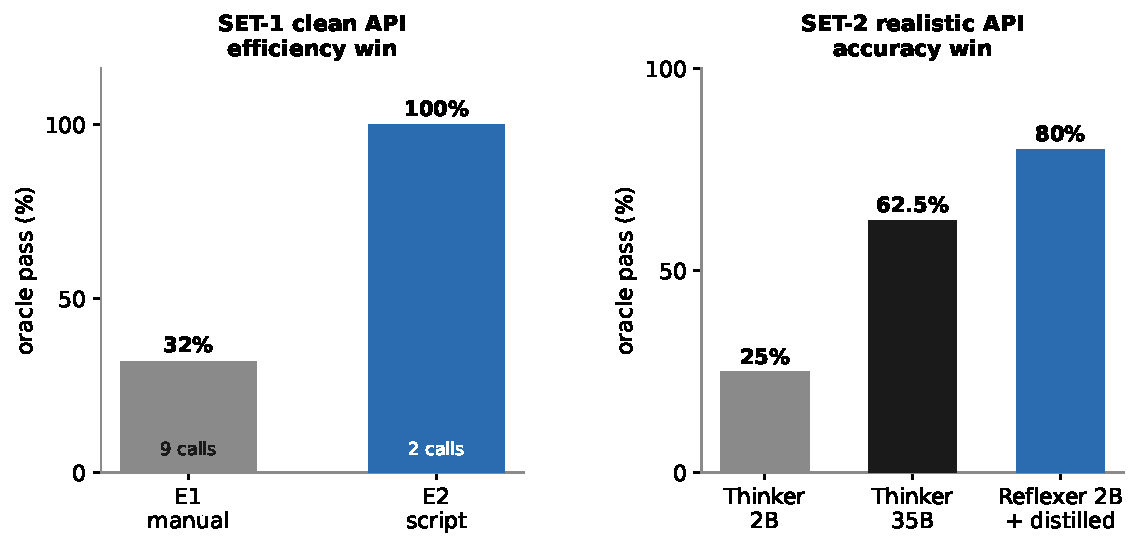
\includegraphics[width=0.95\textwidth]{fig_spectrum.pdf}
  \caption{The reflexer's benefit scales with discovery difficulty: an efficiency
  win on a clean API, an accuracy win on a realistic one.}
  \label{fig:spectrum}
\end{figure}

\section{The limit of scale}
\label{sec:p4}

If a small free-form model fails SET-2, the obvious response is to use a bigger
one. This section shows where that response stops working, the result the thesis
is built around.

A 35B reasoning thinker (\texttt{qwen3.6-35b}) was run on the hardest SET-2
slices: the last three tasks (\textbf{3/3}, \texttt{set2-thinker-qwen3.6-35b-*.json})
and the five hardest excluding those (\textbf{2/5}, \texttt{set2-thinker-35b-hard5.txt}),
for \textbf{5/8 (62.5\%)} combined, at roughly nine calls and 17--20 seconds per
task, off-device. The 35B clearly beats the 2B, but the manner of its failures
is the point. They are not \emph{discovery} failures. The 35B reliably finds the
right namespace and key by exploring the API (\texttt{list}, \texttt{grep},
\texttt{get}, then \texttt{put}). Its failures are \emph{encoding semantics}
(Table~\ref{tab:limit}).

\begin{table}[t]
\centering
\caption{The 35B thinker's SET-2 failures are conventions, not discovery. These
values are not derivable from the API; the model guesses, and is wrong.}
\label{tab:limit}
\begin{tabular}{lcc}
\toprule
Task & Correct value & 35B produced \\
\midrule
``largest font'' & \texttt{font\_scale "1.30"} & \texttt{"1.5"} \\
``DND total silence'' & \texttt{zen\_mode 2} & \texttt{1} \\
``DND important only'' & \texttt{zen\_mode 1} & \texttt{2} \\
\bottomrule
\end{tabular}
\end{table}

This separates two kinds of difficulty by what scale can fix.
\textbf{Discovery}, knowing \emph{which} namespace and key, is solvable by
exploration, and the 35B does it. \textbf{Encoding semantics}, knowing what the
enum value \texttt{2} means or what number is ``largest'', is \emph{not
discoverable} from the API at all, and even a 35B guesses and is wrong about half
the time. The \texttt{zen\_mode} error is especially telling: the model makes the
\emph{same} mistake every time it is asked, which marks a consistent gap in what
the model knows rather than sampling noise. \textbf{Scale rescues discovery; scale
cannot rescue undiscoverable conventions.} That knowledge exists only in a
distilled pattern, which is what the next section supplies.

\begin{figure}[t]
  \centering
  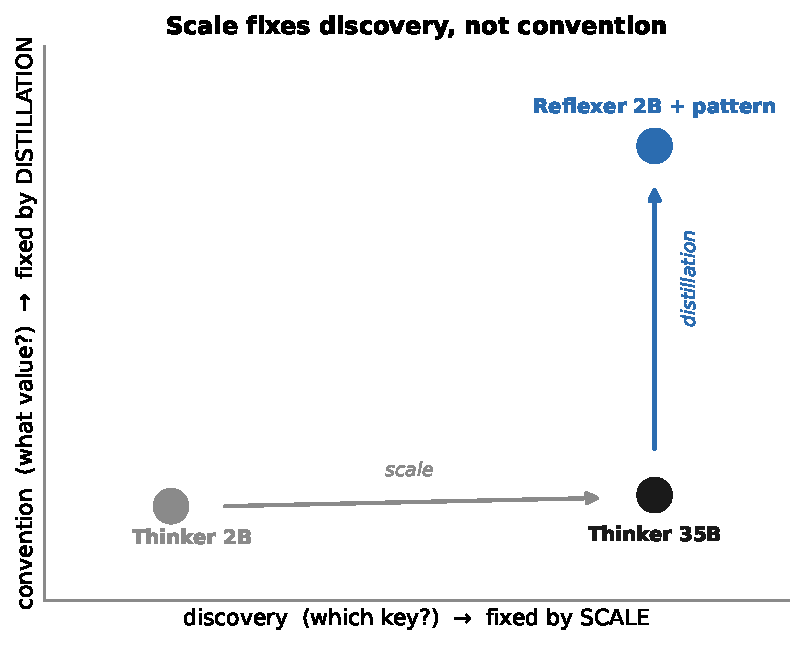
\includegraphics[width=0.72\textwidth]{fig_discovery.pdf}
  \caption{Why a distilled pattern beats a $17\times$ larger model on the
  realistic API: the bottleneck is undiscoverable convention, not reasoning.}
  \label{fig:discovery}
\end{figure}

\section{Closing the loop: cold-start distillation and teacher quality}
\label{sec:p5}

The convention knowledge that no model discovers can be supplied once, offline,
by a teacher. We test this in the hardest honest setting: \emph{cold-start}
distillation, in which the teacher is given only the skill documentation and the
API schema (never any task or its gold outcome), and must mint the patterns from
documentation and prior knowledge alone. The 2B reflexer then applies those
patterns on the single-setting tasks, scored by the same end-state oracle.

With a capable cloud teacher (Claude Sonnet 4.6), the reflexer rises from the
free-form 25\% to \textbf{19/25 (76\%)} on the initial cold-start run, and to
\textbf{20/25 (80\%)} under the key-matched mapping used for the teacher
comparison below.% TODO reconcile 19 vs 20: confirm whether one task flipped between the E3/E4 run and the key-matched re-run; report the single authoritative figure.
\ The teacher encoded the very conventions the larger in-context thinker got
wrong (including \texttt{zen\_mode = 2} for total silence), and honestly flagged
the two it was unsure of (\texttt{font\_scale} ``largest'' and
\texttt{wifi\_sleep\_policy} ``never''), which are genuinely device- or
version-specific and not derivable from documentation
(\texttt{set2-reflexer-qwen-3.5-2b-*.json}). A distilled pattern minted without
ever seeing a task therefore beats a $17\times$ larger model that reasons over
the live API, because it carries knowledge the API does not expose.

Because the teacher is a swappable component, its quality should propagate to the
student, and it does. Repeating the cold-start distillation with a \emph{local}
35B teacher (\texttt{qwen3.6-35b}) under an identical prompt, then running the
\emph{same} 2B reflexer on each teacher's patterns, gives Table~\ref{tab:teacher}.

\begin{table}[t]
\centering
\caption{Teacher quality propagates to the student: $-20$ points from the weaker
teacher, on the same reflexer and tasks (key-matched mapping, 25 single-setting
tasks). Sources: \texttt{patterns\_distilled.json} (cloud) vs
\texttt{patterns\_distilled\_pi.json} (local); \texttt{set2-reflexer-qwen-3.5-2b-*}.}
\label{tab:teacher}
\begin{tabular}{lccc}
\toprule
Teacher (distiller) & Structure (keys/ns) & Conventions correct & Reflexer pass \\
\midrule
Sonnet 4.6 (cloud) & 32/32, 0 errors & $\sim$5/7 critical & \textbf{20/25 (80\%)} \\
qwen3.6-35b (local) & 32/32, 0 errors & $\sim$2/7 critical & 15/25 (60\%) \\
\bottomrule
\end{tabular}
\end{table}

Both teachers are perfect on \emph{structure} (every key, every namespace), so
discovery is easy for either. They diverge on \emph{conventions}. The local 35B
baked in its own wrong priors: \texttt{zen\_mode} total-silence as \texttt{1}
(the same error it made as a thinker, a consistent gap), \texttt{location\_mode}
high-accuracy collapsed to a three-value enum, a wrong brightness worked example,
and an over-verbose \texttt{airplane} encoding that induced \emph{collateral
edits} in the student (the 2B then toggled Wi-Fi and Bluetooth too, failing the
no-collateral oracle). It also reported ``all verified'' while silently wrong,
where the cloud teacher flagged its uncertainty. The lesson is operational:
cold-start distillation should use the strongest available teacher as a one-time
step; a weak local teacher is a weak distiller, and the cheap reflexer faithfully
executes whatever priors it inherits. The two conventions both teachers miss
point at the remaining lever, session-based grounding on the real device, which
Chapter~\ref{ch:discussion} returns to.

\section{Coverage: what fraction of real use-cases this addresses}
\label{sec:coverage}

Binding accuracy is meaningful only against a denominator of real demand. Mapping
the skill library against the on-device use-cases that Google (Gemini Nano via
AICore) and Apple (Apple Intelligence, App Intents) target shows that the
reflexer's natural territory is the \emph{deterministic head}: single-command
device and media control, smart-home toggles, system and timer operations, and
parameterized reads with clear verbs. Apple's App Intents are, in effect, the
same construct as a distilled pattern, a pre-declared parameterized action the
on-device model fills rather than invents, which is independent validation of
the executioner design. What the reflexer does not cover, by design, escalates to
the thinker: multi-intent requests, conversation and planning, and anything
outside an installed skill. The qualitative coverage mapping is documented in
\texttt{docs/research/ondevice\_usecases\_pixel\_apple.md}.

\section{The honest bottleneck: routing, not binding}
\label{sec:routing}

This thesis has held routing fixed in order to isolate binding, and binding is
effectively solved on the deterministic slice (96--100\%). End-to-end coverage,
however, is the product of routing and binding, and routing is the limiter. On
creative, well-designed skills, routing reaches about 85\%; on overlapping skills
it falls to 66--68\%, so realistic single-intent coverage today is roughly
65--85\%, set almost entirely by the router
(\texttt{routing\_ablation\_report.md}; \texttt{findings\_retrieval\_and\_selection.md}).
Decomposed, retrieval is not the bound (the correct candidate is usually in the
top-3); the bound is \emph{selection}: the router picks the wrong sibling within
or across skills, and selection does not improve with selector scale, only with
better prompting. Stating this plainly is part of the contribution: the binding
ceiling is reached, and the open problem for a shippable system is the router.

\section{Economics: when reflexing is worth it}
\label{sec:economics}

The architecture is ultimately a cost argument, so it should be settled as cost
accounting. A pattern is a frozen answer shape: the reflexer never \emph{solves}
the task, it fills in a solution found once, which is why a 2B can match a 35B on
it. In distillation terms the large model is the \emph{teacher} that mints the
pattern once, offline, and the reflexer is the \emph{student} that runs it
forever, on-device; the teacher's cost is paid at distillation time, not at
inference time, and, unlike a fine-tune, the symbolic pattern stays
plug-and-play.

\begin{table}[t]
\centering
\caption{Order-of-magnitude cost model. Break-even is reached at roughly ten
invocations, before counting the size, latency, and on-device-feasibility
advantages. Source: \texttt{findings\_thinker\_vs\_reflexer.md} \S9.}
\label{tab:economics}
\begin{tabular}{lll}
\toprule
 & One-time (distill) & Per-invocation (forever) \\
\midrule
Reflexer atom & $\sim$5--15k teacher tokens + brief review & $\sim$0.3k tokens, $<$1 s, fits on-device (2B) \\
Thinker (big) & 0 & $\sim$1.3k tokens, $\sim$6.4 s, off-device (35B) \\
\bottomrule
\end{tabular}
\end{table}

With per-invocation savings of roughly 1k tokens and a one-time cost near 10k
tokens to mint an atom, distillation breaks even at about ten invocations
(Table~\ref{tab:economics}), before the $\sim$17$\times$ per-token size discount,
the drop from 6.4\,s to under a second, and the fact that the reflexer fits
on-device while the 35B does not. For a head intent invoked thousands of times
this is a $100$--$1000\times$ net win; for a tail intent invoked once it never
amortizes and should be routed to the thinker. The right design is therefore not
``reflexer or bigger model or better router'' but all three in their places:
distill the high-frequency head, spend the big model as the offline teacher and
the tail fallback, and fund the router regardless, because it gates both tiers.

\section{Summary}
\label{sec:eval-summary}

The five results compose into one line. A small model cannot drive a realistic
device API by reasoning (25\%), and scaling the model up to 35B rescues
\emph{discovery} but not \emph{convention} (62.5\%, with consistent
encoding errors). A pattern distilled once by a strong teacher carries exactly
that convention, lifting a 2B reflexer to 76--80\% at one on-device call, and the
quality of that teacher propagates directly to the student ($80\%$ vs $60\%$). On
the clean API the same abstraction is instead an efficiency win
($+65$ points, 2 calls versus 9). Binding, in short, is solved by distillation
rather than scale; the remaining open limit is routing. The next chapter draws
out what this means for design, for productization, and for the validity of the
claims.
           % drafted
\chapter{Discussion}
\label{ch:discussion}

\section{What the results mean}
\label{sec:d-meaning}

The five results of Chapter~\ref{ch:eval} compose into a single claim with a sharp
boundary. On the repeatable head of on-device tasks, a 2B reflexer with a
distilled pattern matches a $17\times$ larger free-form thinker, because the
reflexer does not solve the task---it replays a solution found once. The boundary
is the distinction the thesis makes precise: model scale buys \emph{discovery},
the search for which namespace and key a request maps to, but it does not buy
\emph{convention}, the device-specific meaning of a value. A 35B thinker explores
the API and finds the right key, then guesses the encoding and is wrong about half
the time, making the \emph{same} mistake every time it is asked
(Section~\ref{sec:p4}). A distilled pattern carries that convention, so a small
model applying it succeeds where the large model reasoning from scratch fails.

This reframes a question usually posed as ``how capable a model do we need'' into
``where does the required knowledge live.'' For discovery, the knowledge is in the
API and a capable model can find it. For convention, the knowledge is in neither
the API nor the model's parameters at any scale tested; it exists only in a
distilled artifact. Once that is seen, the economics follow directly
(Section~\ref{sec:economics}): pay a strong teacher once to externalize the
convention, and a cheap student applies it forever. The teacher-quality result
sharpens the recipe---because the student faithfully executes whatever convention
the teacher encoded, a weak teacher bakes in wrong priors, so the one-time
distillation step should use the strongest available teacher
(Section~\ref{sec:p5}).

\section{Implications for productization}
\label{sec:d-product}

The architecture suggests a clear product shape and an equally clear set of
blockers. The defensible first version is a \emph{deterministic-intent
accelerator}: the high-frequency, unambiguous head---media and device control,
smart-home toggles, timers, system actions---served on-device by the reflexer at
near-100\% binding, with the thinker as a safety net for everything else. This is
the slice where the value is highest and the risk is lowest, and it coincides with
the on-device sweet spot that the Pixel and Apple use-case mapping identifies
(Section~\ref{sec:coverage}).

The blockers are ranked by how much they gate a shippable system. \emph{Routing
reliability} is first: end-to-end accuracy is the product of routing and binding,
binding is solved, and routing at 66--85\% is below what users tolerate for an
assistant (Section~\ref{sec:routing}); a misroute to the wrong action is the
dangerous failure, worse than a refusal. \emph{Cold-start data and authoring cost}
is second: each skill needs a pattern set, and patterns must be distilled and,
ideally, kept current as device APIs change; the distillation pipeline is what
makes this scale. \emph{Composite slot extraction} is third: multi-step routines
that need values produced at run time are the high-value automation surface and
remain the reflexer's weak point. None of these is a flaw in the executioner idea;
they are the engineering distance between a validated mechanism and a product.

\section{Threats to validity}
\label{sec:d-threats}

Three caveats must travel with the headline numbers, and the thesis states them
rather than burying them.

First, the comparison is \emph{conditional on a constrained task}. The reflexer is
handed the command template and only fills slots, which is strictly easier than
free-form generation. The claim is therefore not that a 2B is more capable than a
35B; it is that on the distillable slice a constrained 2B executor reaches the
same binding accuracy at a fraction of the cost. Read as a capability claim it
would be wrong; read as a systems claim it is what the numbers support.

Second, \emph{coverage is limited to distilled intents}. The 100\% binding figure
is a ceiling that applies only when a pattern exists and routing has selected it.
For intents with no pattern, the system falls back to the thinker, and the
reflexer contributes nothing. The approach is a head strategy by construction; its
value depends on the workload actually having a repeatable head, which the
coverage mapping argues it does.

Third, the strongest results rest on a \emph{small number of comparisons on
purpose-built benchmarks} with specific models. SET-2 is realistic but is a model
of the Android settings surface, not the full device; the 35B is one large model,
not a survey of large models; and two runs of the cold-start reflexer disagreed by
one task (19 versus 20 of 25), which the thesis reports rather than reconciles. The
qualitative pattern---scale fixes discovery but not convention, distillation fixes
both, teacher quality propagates---is robust across the experiments, but the exact
percentages should be read as evidence for that pattern rather than as universal
constants.

\section{Limitations}
\label{sec:d-limits}

Beyond the threats to validity, four limitations bound the work. The router is
evaluated but not solved; it is named as the open bottleneck rather than fixed.
Composite slot-filling is identified as weak but not repaired. Both teachers,
cloud and local, miss the genuinely undiscoverable conventions (the version- or
OEM-specific values), which no cold-start teacher can recover and which require
observing the real device. And the reflexer's residual application errors---using
an enum label instead of its code, or mis-doing brightness arithmetic---point to a
value-transform step that is currently left to the model. Each of these limitations
maps onto a concrete next step rather than an open research question, which the
next chapter sets out.
           % drafted
\chapter{Conclusion and Future Work}
\label{ch:conclusion}

\section{Summary}
\label{sec:c-summary}

This thesis asked how much language model reliable on-device action requires, and
answered it through A.L.F.R.E.D., a two-tier local-first middleware that routes
each request to a tiny reflexer or a heavier thinker. The five research questions
are settled by the evaluation.

\emph{On scale versus distillation} (RQ1), a 2B reflexer with a distilled pattern
matches a 35B free-form thinker on binding (both 100\% balanced), while the same
2B without a pattern reaches 30\%; the pattern is worth roughly $17\times$ the
parameters. \emph{On the spectrum} (RQ2), the abstraction is an efficiency win on
a clean API (a $+65$-point oracle gain at two calls instead of nine) and an
accuracy win on a realistic one. \emph{On the limit of scale} (RQ3), a 35B thinker
rescues discovery but not convention, failing device encodings consistently, while
a distilled pattern supplies exactly that convention. \emph{On teacher quality}
(RQ4), end-to-end student accuracy tracks the teacher: a cloud teacher's patterns
score 80\% against a local teacher's 60\% on the same reflexer and tasks. \emph{On
coverage and routing} (RQ5), the reflexer's territory is the deterministic head
that on-device assistants target, and the open bottleneck is routing, not binding.

The contribution, stated once more in plain terms: \textbf{on a real device API,
scale buys discovery but not undiscoverable convention; distillation buys the
convention; and a small reflexer applies it at a fraction of the cost.} The
executioner paradigm is validated through the full teacher-to-student loop, and
its central mechanism, compressing a teacher's device knowledge into an
inspectable symbolic pattern rather than into student weights, is the thesis's
main idea.

\section{Future work}
\label{sec:c-future}

The limitations of Chapter~\ref{ch:discussion} map onto five concrete next steps,
ordered by leverage.

\paragraph{Session-based device grounding.} Both teachers miss the genuinely
undiscoverable conventions because cold-start distillation gives them no way to
check a value against reality. Granting the teacher read-only access to the real
device, so it observes actual codes before committing an encoding, would convert
those guesses into facts and close the remaining convention errors. The integrity
rule carries over: ground on the device or a development split, never on the
evaluation gold.

\paragraph{Deterministic value transforms.} The reflexer's residual errors are
arithmetic and enum-lookup mistakes (percent-to-0--255, label-to-code). Moving
these transforms out of the model and into a small deterministic function inside
the pattern removes them for both the teacher and the student, and is a bounded
engineering change.

\paragraph{The router.} The evaluation localizes the open bottleneck precisely:
retrieval places the correct candidate in the top-3, but selection picks the wrong
sibling, and selection does not improve with selector scale. The next investment
is sibling discrimination, whether through better selection prompting or a learned
selector over behavioural signals, since the router gates both tiers.

\paragraph{Iterative, grounded distillation.} The cold-start patterns can be run,
executed on a real device, and re-distilled from the observed failures over two to
three rounds, lifting a weak local teacher toward cloud quality without a larger
model. This iteration lives entirely in the offline learning phase; the run-time
reflex remains a single pass over a frozen pattern, so the simplicity that makes
the reflexer deployable is preserved by construction, with a minimality check each
round to stop patterns accreting special cases.

\paragraph{Authoring and personalization at scale.} Longer-term, mining a user's
own repeated trajectories into candidate patterns would extend coverage beyond
hand-authored skills, and a privacy-preserving sharing layer would let patterns be
exchanged without leaking personal data. A parametric alternative, fine-tuning a
very small model on the pattern conventions, is a path worth measuring against the
symbolic approach, trading inspectability for a smaller artifact.

\paragraph{Development substrate.} All of the above extensions are intended to be
built inside the \textbf{Pi coding-agent framework}~\citep{pi-agent} on which the
thinker already runs (Section~\ref{sec:thinker}). Consolidating the reflexer's
future work in the same minimal, transparent environment keeps the executor and
the agent loop on one runtime, tool surface, and instrumentation path, which lowers
the cost of the iterate-and-measure loop the rest of this section depends on.

\section{Closing}
\label{sec:c-closing}

The shift toward on-device assistants raises a practical question that this thesis
takes seriously: not how powerful a model can be, but how little model an action
actually needs once its knowledge is placed where it belongs. The answer found
here is that a great deal of on-device action is not a reasoning problem at all. It
is a knowledge-placement problem, and once the convention is distilled into a
pattern, a small model executing a frozen reflex is enough.
           % drafted

% ---------------------------------------------------------------- back matter
\bibliographystyle{apacite}
\bibliography{references}

\end{document}
